\message{ !name(processo.tex)}\documentclass[a4paper,12pt, oneside]{book}

% \usepackage{fullpage}
\usepackage[italian]{babel}
\usepackage[utf8]{inputenc}
\usepackage{amssymb}
\usepackage{amsthm}
\usepackage{graphics}
\usepackage{amsfonts}
\usepackage{listings}
\usepackage{amsmath}
\usepackage{amstext}
\usepackage{engrec}
\usepackage{rotating}
\usepackage{verbatim}
\usepackage[safe,extra]{tipa}
%\usepackage{showkeys}
\usepackage{multirow}
\usepackage{hyperref}
\usepackage{microtype}
\usepackage{fontspec}
\usepackage{enumerate}
\usepackage{braket}
\usepackage{marginnote}
\usepackage{pgfplots}
\usepackage{cancel}
\usepackage{polynom}
\usepackage{booktabs}
\usepackage{enumitem}
\usepackage{framed}
\usepackage{pdfpages}
\usepackage{pgfplots}
\usepackage{algorithm}
% \usepackage{algpseudocode}
\usepackage[cache=false]{minted}
\usepackage{mathtools}
\usepackage[noend]{algpseudocode}

\usepackage{tikz}\usetikzlibrary{er}\tikzset{multi  attribute /.style={attribute
    ,double  distance =1.5pt}}\tikzset{derived  attribute /.style={attribute
    ,dashed}}\tikzset{total /.style={double  distance =1.5pt}}\tikzset{every
  entity /.style={draw=orange , fill=orange!20}}\tikzset{every  attribute
  /.style={draw=MediumPurple1, fill=MediumPurple1!20}}\tikzset{every
  relationship /.style={draw=Chartreuse2,
    fill=Chartreuse2!20}}\newcommand{\key}[1]{\underline{#1}}
  \usetikzlibrary{arrows.meta}
  \usetikzlibrary{decorations.markings}
  \usetikzlibrary{arrows,shapes,backgrounds,petri}
\tikzset{
  place/.style={
        circle,
        thick,
        draw=black,
        minimum size=6mm,
    },
  transition/.style={
    rectangle,
    thick,
    fill=black,
    minimum width=8mm,
    inner ysep=2pt
  },
  transitionv/.style={
    rectangle,
    thick,
    fill=black,
    minimum height=8mm,
    inner xsep=2pt
    }
  } 
\usetikzlibrary{automata,positioning}
\usepackage{fancyhdr}
\pagestyle{fancy}
\fancyhead[LE,RO]{\slshape \rightmark}
\fancyhead[LO,RE]{\slshape \leftmark}
\fancyfoot[C]{\thepage}


\title{Processo e Sviluppo del Software}
\author{UniShare\\\\Davide Cozzi\\\href{https://t.me/dlcgold}{@dlcgold}}
\date{}

\pgfplotsset{compat=1.13}
\begin{document}

\message{ !name(processo.tex) !offset(-3) }

\maketitle

\definecolor{shadecolor}{gray}{0.80}
\setlist{leftmargin = 2cm}
\newtheorem{teorema}{Teorema}
\newtheorem{definizione}{Definizione}
\newtheorem{esempio}{Esempio}
\newtheorem{corollario}{Corollario}
\newtheorem{lemma}{Lemma}
\newtheorem{osservazione}{Osservazione}
\newtheorem{nota}{Nota}
\newtheorem{esercizio}{Esercizio}
\algdef{SE}[DOWHILE]{Do}{doWhile}{\algorithmicdo}[1]{\algorithmicwhile\ #1}
\tableofcontents
\renewcommand{\chaptermark}[1]{%
  \markboth{\chaptername
    \ \thechapter.\ #1}{}}
\renewcommand{\sectionmark}[1]{\markright{\thesection.\ #1}}
\newcommand{\floor}[1]{\lfloor #1 \rfloor}
\newcommand{\MYhref}[3][blue]{\href{#2}{\color{#1}{#3}}}%
\chapter{Introduzione}
\textbf{Questi appunti sono presi a lezione. Per quanto sia stata fatta
  una revisione è altamente probabile (praticamente certo) che possano
  contenere errori, sia di stampa che di vero e proprio contenuto. Per
  eventuali proposte di correzione effettuare una pull request. Link: }
\url{https://github.com/dlcgold/Appunti}.\\
\textbf{Le immagini presenti in questi appunti sono tratte dalle slides del
  corso e tutti i diritti delle stesse sono da destinarsi ai docenti del corso
  stesso}.
\chapter{Metodi Agili}
I \textit{metodi agili} sono stati definiti per rispondere all'esigenza di dover
affrontare lo sviluppo di software in continuo cambiamento. Durante lo sviluppo
si hanno vari passaggi:
\begin{itemize}
  \item comprensione dei prerequisiti
  \item scoperta di nuovi requisiti o cambiamento dei vecchi
\end{itemize}
Questa situazione rendeva difficile lo sviluppo secondo il vecchio metodo
\textit{waterfall} (a cascata) portando al fallimento di diversi progetti.\\
I \textit{metodi agili} ammettono che i requisiti cambino in modo ``naturale''
durante il processo di sviluppo software e per questo assumono un modello di
processo \textit{circolare}, con iterazioni della durata di un paio di settimane
(figura \ref{agile}). Potenzialmente dopo un'iterazione si può arrivare ad un
prodotto che può essere messo ``in produzione''. Dopo ogni rilascio si
raccolgono \textit{feedback} per poter rivalutare i requisiti e migliorare il
progetto.\\
\begin{figure}
  \centering
  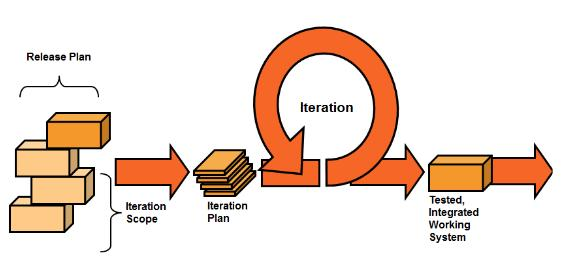
\includegraphics[scale = 0.6]{img/agile.jpg}
  \caption{Rappresentazione grafica del modello agile. I blocchi a sinistra
    rappresentano i requisiti (da sviluppare secondo una certa priorità). Lo
    sviluppo si articola tramite varie iterazioni che porta ogni volta ad
    aggiungere una parte al prodotto finale (ogni iterazione produce, a partire
    da un certo requisito, un parte di
    prodotto di qualità già definitiva, con testing, documentazione
    etc$\ldots$)}
  \label{agile}
\end{figure}
Si hanno quindi aspetti comuni nei metodi agili e nel loro processo:
\begin{itemize}
  \item enfasi sul team, sulla sua qualità e sulla sua selezione
  \item il team è \textit{self organizing}, si da importanza ai vari membri del
  team dato che non esiste un \textit{manager} ma
  è il team stesso a gestire lo sviluppo
  \item enfasi al pragmatismo, focalizzandosi su una documentazione
  efficace evitando di produrre documenti inutili e difficili da mantenere
  \item enfasi sulla comunicazione diretta, sostituendo i documenti suddetti con 
  meeting e riunioni periodiche
  \item enfasi sull'idea che nulla sia definitivo: la perfezione non deve essere 
  seguita fin da subito ma saranno gli step a portare al
  raggiungimento di una perfezione finale (anche dal punto di vista del design)
  \item enfasi sul controllo costante della qualità del prodotto, anche tramite
    \begin{itemize}
      \item \textit{continuous testing} grazie al quale un insieme
  di test viene eseguito in modo automatico dopo ogni modifica
      \item \textit{analisi statica e dinamica} del codice al fine di trovare difetti
  nello stesso
      \item \textit{refactoring}
    \end{itemize}

\end{itemize}
I metodi agili sono molto ``elastici'' e permettono la facile
  definizione di nuovi metodi facilmente adattabili al singolo progetto.
\section{Scrum}
Uno dei più famosi, tra i vari \textit{metodi agili}, è \textbf{scrum} (figura
\ref{scrum}).\\
In questo caso la parte di sviluppo e iterazione prende il nome di
\textit{sprint} ed ha una durata variabile tra una e quattro settimane, per avere
un rilascio frequente e una veloce raccolta di feedback. I requisiti sono
raccolti nel cosiddetto \textit{product backlog}, con priorità basata sulla base
delle indicazioni del committente. Ad ogni \textit{sprint} si estrae dal
\textit{product backlog} lo \textit{sprint backlog}, ovvero il requisito (o i
requisiti) da implementare nello \textit{sprint}. Lo \textit{sprint backlog}
viene analizzato nel dettaglio producendo i vari \textit{backlog items}, ovvero
le singole funzionalità che verranno implementate nello \textit{sprint}. Si
ottiene quindi di volta in volta un pezzo di prodotto finale, testato e
documentato. Durante le settimane di \textit{sprint} si effettua anche un meeting
giornaliero utile per mantenere alti i livelli di comunicazione e visibilità
dello sviluppo. Durante il meeting ogni sviluppatore risponde a tre domande:
\begin{enumerate}
  \item Cosa è stato fatto dall'ultimo meeting?
  \item Cosa farai fino al prossimo meeting?
  \item Quali sono le difficoltà incontrate?
\end{enumerate}
L'ultimo punto permette la cooperazione tra \textit{team members}, consci di cosa
ciascuno stia facendo.\\
\begin{figure}
  \centering
  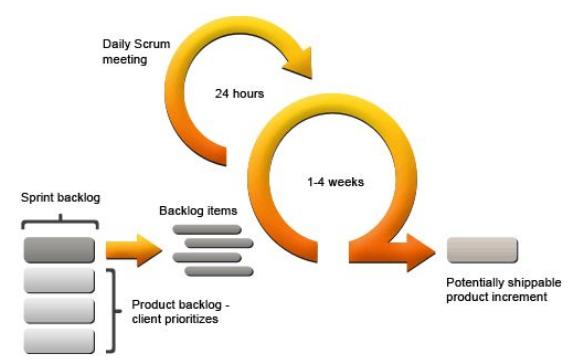
\includegraphics[scale = 0.6]{img/scrum.jpg}
  \caption{Rappresentazione grafica del processo scrum}
  \label{scrum}
\end{figure}
Durante il processo \textit{scrum} si hanno quindi tre ruoli:
\begin{enumerate}
  \item il \textbf{product owner}, il committente che partecipa tramite feedback
  e definizione dei requisiti
  \item il \textbf{team} che sviluppa
  \item lo \textbf{scrum master} che controlla la correttezza di svolgimento del processo scrum 
\end{enumerate}
Essi collaborano nelle varie fasi:
\begin{itemize}
  \item product owner e team collaborano nella definzione dei backlog e nella
  loro selezione ad inizio \textit{sprint}
  \item durante lo \textit{sprint} lavora solo il team
  \item nello studio del risultato collaborano tutti coloro che hanno un
  interesse diretto nel progetto (team, product owner e stakeholders) 
\end{itemize}
\textit{Lo scrum master interagisce in ogni fase, fase che viene comunque
  guidata tramite meeting}:
\begin{itemize}
  \item \textbf{sprint planning meeting}, ad inizio \textit{sprint}
  \item \textbf{daily scrum meeting}, il meeting giornaliero
  \item \textbf{sprint review meeting}, in uscita dallo \textit{sprint} per lo
  studio dei risultati
  \item \textbf{sprint retrospective meeting}, in uscita dallo \textit{sprint}
  per lo studio tra i membri del team di eventuali migliorie al processo e allo
  sviluppo del prodotto (anche dal punto di vista delle tecniche e delle
  tecnologie)
\end{itemize}
\section{Extreme Programming}
Un altro tipo di metodo agile è l'\textit{extreme programming} (figura
\ref{extreme}), ormai poco usato. I requisiti prendono i nomi di
\textit{stories}, delle narrazioni in cui l'attore (futuro utente del sistema) cerca 
di svolgere un compito. Vengono
scelti quindi \textit{stories} per la prossima iterazione, dove si hanno testing
e revisione continua. Le release di ogni iterazione vengono catalogate per
importanza (con anche la solita collezione di feedback). In \textit{extreme
  programming} si hanno davvero molte pratiche:
\begin{itemize}
  \item The Planning Game
  \item Short Releases
  \item Metaphor
  \item Simple Design
  \item Refactoring
  \item Test-First Design
  \item Pair Programming
  \item Collective Ownership (codice condiviso da tutti senza alcun owner, con
  tutti in grado di effettuare modifiche)
  \item Continuous Integration
  \item 40-Hour Week
  \item On-Site Customer
  \item Coding Standard (per avere il collective ownership avendo un solo
  standard di codifica comune a tutti)
  \item Open workspace
\end{itemize}
\begin{figure}
  \centering
  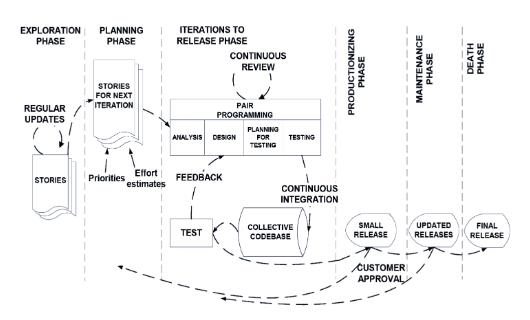
\includegraphics[scale = 0.7]{img/extreme.jpg}
  \caption{Rappresentazione grafica dell'extreme programming}
  \label{extreme}
\end{figure}
\chapter{DevOps}
Nel tempo si è passato dal \textit{modello waterfall} (dove tutto era definito
ad inizio progetto) al \textit{modello agile}. Negli ultimi tempi si è
sviluppato un altro metodo, chiamato \textbf{DevOps}, dove anche la parte di
\textit{operation} deve essere agile: il rilascio in produzione e il
\textit{deployment} devono essere agili quanto lo sviluppo. Amazon, Netflix,
Facebook e molte altre società già adottano le pratiche \textit{DevOps.}\\
Nel \textit{DevOps} i team di sviluppo e operation sono indipendenti tra loro,
diminuendo il costo di impegno necessario al team di sviluppo per la parte di
deployment (che viene resa anche più sicura grazie alla diminuzione
dell'intervento umano in favore di automazioni). Inoltre, avendo i due team dei
tempi di lavoro diversi, si riesce a prevenire ritardi causati dalla non
organicità delle operazioni.\\
DevOps promuove la collaborazione tra di due team al fine di ottenere una sorta
di team unico che curi sia sviluppo che operation.\\
DevOps include quindi diversi processi che vengono automatizzati:
\begin{itemize}
  \item Continuous Development
  \item Continuous Integration
  \item Continuous Testing
  \item Continuous Deployment (anche con tecnologie di virtualizzazione e
  con l'uso di \textit{container} in \textit{ambiente cloud})
  \item Continuous Monitoring
\end{itemize}
Con DevOps il feedback arriva in primis dal software (i tool di
\textit{monitor}) inoltre il focus viene spostato sui processi automatici.\\
Nel DevOps si introducono nuovi ruoli:
\begin{itemize}
  \item il \textbf{DevOps Evangelist}, simile allo \textit{scrum master},
  supervisiona l'intero processo di DevOps
  \item l'\textbf{automation expert}, dedicato a curare gli aspetti di
  automatismo 
  \item un \textbf{Security Engineer}
  \item un \textbf{Software Developer}, nonché \textbf{Tester}
  \item un \textbf{Quality Assurance} che verifica la qualità del prodotto
  rispetto ai requisiti
  \item un \textbf{Code Release Manager} che si occupa sull'infrastruttura e
  sul deploy della release
\end{itemize}
Il DevOps (figura \ref{devops}) si basa su sei principi base:
\begin{enumerate}
  \item \textbf{Customer-Centric Action}, ovvero il committente è al centro
  dell'azione 
  \item \textbf{End-To-End Responsibility}, ovvero il team gestisce interamente
  il prodotto, avendone responsabilità totale
  \item \textbf{Continuous Improvement}, ovvero cercare continuamente di
  migliorare senza sprechi il prodotto finale e i servizi
  \item \textbf{Automate everything}, ovvero cercare di automatizzare l'intera
  infrastruttura di processo, dalle attività di testing e integrazione fino ad
  arrivare alla costruzione della release e del deployment
  \item \textbf{Work as one team}, ovvero unificare tutti gli aspetti sotto un
  unico team o comunque con due team che collaborano fortemente come se fossero
  uno 
  \item \textbf{Monitor and test everything}, ovvero testare e monitorare
  costantemente il prodotto
\end{enumerate}
\textit{Il quarto e il sesto punto sono i due punti tecnici principali}.
\begin{figure}
  \centering
  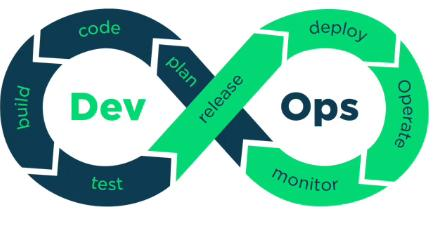
\includegraphics[scale = 0.6]{img/devops.jpg}
  \caption{Rappresentazione famosa del \textit{lifecycle} di DevOps, con le due
    parti, con le relative parti fondamentali, di sviluppo e operation distinte
    dai colori ma unite in un singolo metodo unico}
  \label{devops}
\end{figure}
\section{Build, Test e Release}
Partiamo dalla parte ``dev'' di DevOps.\\
Bisogna pensare a questi step in ottica di automatismo vicina al DevOps. \\
Innanzitutto bisogna introdurre i sistemi di \textbf{version control}, in primis
\textbf{Git}, un sistema di version control \textbf{distribuito}, dove ogni
utente ha una copia della repository (con la storia dei cambiamenti), con la
quale interagisce tramite \textit{commit} e \textit{update}. Esiste poi una
repository lato server per permettere di condividere i vari cambiamenti tramite
sincronizzazione.\\
\textbf{Git} permette anche lo sviluppo \textit{multi-branch} per permettere di
lavorare su più branch, pensando allo sviluppo separato dove ogni branch alla
fine può essere unito (\textit{merge}) con quello principale (solitamente
chiamato \textit{master}). Un altro branch standard è quello di sviluppo, detto
\textit{develop}. Un altro ancora è quello detto \textit{hotfix}, per le
modifiche più urgenti, che vive in uno stadio intermedio tra i due
sopracitati, prima ancora del branch \textit{develop}. Volendo ciascuna feature
può essere creata in un branch dedicato. Si procede con le versioni
``merge-ndo'' quando necessario, ``step by step'' fino ad un branch
\textit{release} per poi andare dopo il testing su \textit{master}. Sul branch
\textit{release} possono essere effettuati fix che poi verranno riportati anche
in \textit{develop}.\\
Lo sviluppo su multi-branch si collega alle operazioni di verifica che possono
essere attivate automaticamente a seconda dell'evoluzione del codice su ogni
branch. Avendo ogni branch una precisa semantica possiamo definire precise
attività di verifica, corrispondenti a \textit{pipelines} precise, solitamente
innescate da un \textit{push} di codice su un certo branch, in modo sia
automatico che manuale. Le pipeline vengono attivate in fase di test di un
componente, in fase di creazione di un sottosistema, di assembramento di un
sistema intero o di deployment in produzione. Si hanno quindi quattro fasi:
\begin{enumerate}
  \item component phase
  \item subsystem phase
  \item system phase
  \item production phase
\end{enumerate}
Spesso le pipelines sono usate
come \textit{quality gates} per valutare se un push può essere accettato in un
certo branch. Una pipeline può essere anche regolata temporalmente, in modo che
avvenga solo ad un certo momento della giornata.
\subsubsection{Component phase e Subsystem phase}
Dove il fuoco è sulla più piccola unità testabile che viene aggiornata (una
classe, un metodo etc$\ldots$) che non può essere eseguita senza l'intero
sistema. In tal caso si può fare:
\begin{itemize}
  \item code review
  \item unit testing
  \item static code analysis
\end{itemize}
Un cambiamento può anche essere testato nell'ambito del sottosistema di cui fa
parte, in tal caso si hanno anche check di prestazioni e sicurezza. Il servizio
però potrebbe essere da testare in isolamento rispetto ad altri servizi, usando
quindi dei \textit{mocks} o degli \textit{stubs}, ovvero creando degli alter ego
dei servizi mancanti in modo che il servizio da testare possa funzionare.
\subsubsection{System phase}
In questo caso si testa l'intero sistema che viene ``deployato'' in ambiente di
test. Si hanno:
\begin{itemize}
  \item integration tests
  \item performance tests
  \item security tests
\end{itemize}
Tutti test che richiedono l'interezza del sistema e sono spesso molto
dispendiosi e quindi bisogna regolare la frequenza di tali test in molti casi
(sfruttando ad esempio la notte).
\subsubsection{Production phase}
Questa fase è legata alla necessità di creare gli artefatti che andranno
direttamente ``sul campo'', ovvero il deployment in produzione. In tale fase
potrebbe essere necessario creare container o macchine virtuali. Si
hanno dei check molto veloci sugli artefatti finali (che non siano per esempio
corretti), dando per assodato che la qualità del codice sia già stata
testata. Si hanno quindi strategie anche di \textit{deployment incrementale},
per cui esistono più versioni del software contemporaneamente con diversa
accessibilità per gli utenti finali (accessibilità che viene man mano
scalata). In tal caso si usano anche vari tool di monitor. Si hanno anche
eventualmente tecniche di \textit{zero downtime} (dove il software non è mai in
uno stato \textit{unstable}).\\
\\
\textbf{Fasi diverse corrispondono a branch diversi}
\section{Deploy, Operate e Monitor}
Studiamo ora la parte ``Ops'' di DevOps.\\
Si studia l'evoluzione automatica del software da una versione all'altra in
produzione. Avanzare di versione in modo \textit{naive} e istantaneo è troppo
rischioso (qualora la nuova versione fosse corrotta non si avrebbe controllo
sull'update) e quindi spesso non attuabile (spesso anche per ragioni tecniche).
Si ha quindi un insieme di tecniche che si basano in primis
sull'\textit{evoluzione incrementale}. Tali tecniche si distinguono in base alla
dimensione su cui sono incrementati:
\begin{itemize}
  \item \textbf{Incremental wrt users:} \textit{Dark launching, Canary releases
    (and User Experimentation)}, ovvero legata agli utenti esposti alla nuova
  release
  \item \textbf{Incremental wrt requests:} \textit{Gradual upgrades/rollout},
  ovvero legata alle richieste per la nuova release
  \item \textbf{Incremental wrt components/replicas:} \textit{Rolling upgrade},
  incentrata sulle componenti che vengono aggiornate
  \item \textbf{Non-incremental with backups:} \textit{Green/blue deployment,
    Rainbow deployment}, non incrementali ma che offrono comunque un backup di
  sicurezza  
\end{itemize}
Tali schemi possono essere usati in un contesto DevOps.\\
Per studiare la prima tipologia (\textit{Incremental wrt users}) abbiamo:
\begin{itemize}
  \item \textbf{Dark launching} che arriva
  dal mondo di Facebook dal 2011. In tale schema 
  l'update è esposto solo ad una parte della popolazione, per la quale viene
  effettuato il deployment per studiare gli effetti (tramite continuous
  monitoring) ed eventuali modifiche e migliorie al software, che infine verrà
  deployato per il resto della popolazione in modo comunque incrementale fino a
  che l'intera popolazione godrà della feature. Spesso usata per front-end 
  \item \textbf{Canary releases}, che studia l'impatto di update relativi al
  back-end
\end{itemize}
Tali schemi spesso sono usati di pari passo per le varie sezioni del software,
nonché possono essere usati in modo intercambiabile.\\
Collegato a questi schemi si ha l'approccio basato sull'\textbf{user
  experimentation}, che non è un reale schema di gestione dell'evoluzione del
software ma è comunque correlato agli schemi sopra descritti. In questo
approccio si studiano diverse varianti del sistema e il loro impatto esponendole
agli utenti (perlomeno ad una sottoparte degli stessi in modo incrementale),
cercando di capire per l'utente cosa sia meglio e come (si ispira 
alla \textit{sperimentazione scientifico}). Si hanno quindi più release diverse,
per parti di popolazione comparabili, tra le quali si sceglierà la migliore.\\
Per la seconda tipologia (\textit{Incremental wrt requests}) si ha una divisione
a seconda delle richieste fatte dagli utenti (esempio un momento d'uso diverso
porta all'uso di componenti diverse), detto \textit{gradual rollout}. Si ha
quindi un \textit{load balancer} che 
permette la coesistenza di due versioni, una nuova e una vecchia, dello stesso
servizio. In modo graduale, partendo da pochissime, si passano le richieste alla
versione nuova per poter studiare e testare la nuova versione (in caso di
problemi il load balancer dirotterà tutte le richieste alla vecchia
versione). Alla fine tutto il traffico sarà diretto verso la nuova versione,
mentre la vecchia verrà dismessa.\\
Per la terza tipologia (\textit{Incremental wrt components/replicas}), si ha lo
schema del \textit{rolling upgrade}, dove l'upgrade non riguarda un singolo
upgrade ma tanti componenti di un sistema distribuito, verificando efficacia
di ogni singolo update tramite il continuous monitoring prima di effettuare
l'upgrade di un'altra componente. La stessa idea su applica anche a diverse
versioni dello stesso prodotto, aggiornandone una prima e poi le altre
progressivamente. Le nuove versioni delle componenti ``upgradate'' devono essere
compatibili con quelle ancora prive di upgrade.\\
Per la quarta tipologia (\textit{Non-incremental with backups}) si ha il
\textbf{blue/green deployment}, dove vengono isolate due copie della stessa
infrastruttura (anche hardware), dove una ospita la versione nuove l'altra la
vecchia. Un router ridireziona le richieste degli utenti verso le due unità e
quella che ospita la nuova 
versione subirà le solite operazioni di test che, se superate, porteranno il
router a direzionare verso quella unità, ignorando la vecchia. Se ci sono
problemi si fa rollback alla vecchia unità che rimane come backup. Questo schema
può essere generalizzato nel \textbf{rainbow deployment} dove il momento di
coesistenza tra le due versioni (se non più versioni) viene prolungato al fine
che vecchie richieste che richiedono una lunga elaborazione vengano elaborate
dall'unità vecchia mentre le nuove dall'unità nuova.\\
\textbf{In ogni caso le applicazioni devono essere costruite per supportare
  tutti questi schemi di deployment (a causa di stati delle applicazioni,
  backward compatibility etc$\ldots$)}
\subsection{Deployable units}
Il caso più tipico in merito alle unità dove fare deployment è il mondo del
\textbf{cloud}, con \textbf{unità virtualizzate e virtual machine (VM)}, dove
magari ogni servizio vive in una diversa VM. Si hanno diversi casi in merito a
questo tipo di deployment:
\begin{itemize}
  \item \textbf{cloud} basato su \textbf{VMs}, dove si ha un'infrastruttura
  gestita dal cloud provider che gestisce l'hardware e l'hypervisor. Ogni VM,
  che sono le nostre unità di deployment, ha
  un sistema operativo arbitrario che lavora con l'hardware mostrato
  dall'hypervisor. Ogni VM avrà una o più applicazioni e fare deployment porterà
  all'update di una o più VM. In alcuni casi si fa deployment di intere VM e in
  altri si modifica il software di una VM già in esecuzione. L'ambiente cloud
  solitamente è \textbf{multi-tenant} (ovvero su una piattaforma unica di un
  provider si hanno più VM di diverse organizzazioni). Una VM è grossa in quanto
  contiene un sistema operativo intero e la loro gestione può quindi essere
  difficoltosa
  \item \textbf{cloud} basato su \textbf{containers} che risolvono il problema
  della grandezza delle VM. In questo caso lo schema è il medesimo ma si ha un
  \textbf{container engine} al posto dell'hypervisor e ogni container non
  contiene l'intero sistema operativo ma solo il minimo necessario al
  funzionamento dell'applicazione (il sistema operativo viene condiviso dalla
  macchina sottostante, riducendo il volume dei singoli containers). In questo
  caso lo schema di update spesso consiste nel distruggere e ricreare i singoli
  containers. Anche qui si ha un contesto \textit{multi-tenant}
  \item \textbf{bare metal}, dove i provider offrono direttamente risorse
  hardware, guadagnando prestazioni ma aumentano anche i costi economici , che
  vengono comunque gestite dal cloud provider. Non si ha 
  virtualizzazione ma accesso diretto alle risorse su cui fare
  deployment. Questa è una soluzione tipicamente \textbf{single-tenant} (sulla
  macchina gira il software di una sola organizzazione)
  \item \textbf{server dedicati}, un metodo ormai superato con difficoltà
  causate dall'uso di script, shell e connessione \textit{ftp} completamente
  autogestiti dall'organizzazione e non da un provider
\end{itemize}
Il deployment ``stile cloud'' non è comunque l'unico possibile. Un esempio
quotidiano è il deployment di app mobile sui vari store, dove il back-end
probabilmente sarà gestito come sopra spiegato mentre l'app in sé viene
rilasciata negli store e sarà l'utente finale a fare il deployment installando
l'app sul proprio device. Le forme di monitoraggio e di feedback sono spesso
diverse e provengono dagli utenti finali stessi.
\subsection{Monitor}
In ambiente cloud ci sono tante soluzioni per il \textbf{monitoring}, ad esempio
lo \textbf{stack di ELK}, formato da:
\begin{itemize}
  \item \textbf{Elasticsearch}
  \item \textbf{Logstash}
  \item \textbf{Kibana}
\end{itemize}
I dati, ad esempio log o metriche d'uso hardware, vengono raccolti e passano da
\textbf{Logstash}, finendo in un database, per la memorizzazione di \textit{time
series} (serie temporali) di dati (questo in primis per le metriche d'uso che
per i log), gestito da \textbf{Elasticsearch} e venendo visualizzati da una
dashboard grafica, gestita da \textbf{Kibana}. Si ha quindi un ambiente di
\textbf{continuous monitoring}.
\subsection{DevOps tools}
Ogni step del DevOps è gestito tramite moderne tecnologie e tools , con varie
alternative per ogni fase (per questo servono figure 
esperte per ogni step). Vediamo qualche esempio (in ottica più spinta ad un
progetto in Java):
\begin{itemize}
  \item code: Git, Svn, Jira, Eclipse
  \item build: Apache Ant, Maven, Gradle
  \item test: JUnit
  \item release: Jenkins, Bamboo
  \item deploy: Pupper, Chef, Ansible, SaltStack
  \item monitor: New Relic, Sensu, Splunk, Nagios
\end{itemize}
\chapter{Risk management}
Partiamo da un semplice esempio:
\begin{esempio}
  Durante lo sviluppo di un progetto software l'unico dev, insoddisfatto del
  salario, che conosceva un modulo di importanza critica lascia la società,
  rallentando in modo serio lo sviluppo del progetto (nonché aumentandone i
  costi, nel tentativo di cambiare il modulo conosciuto solo dal dev) fino a
  farlo uscire troppo in ritardo rispetto, ad esempio, alle 
  opportunità di marketing a cui puntava.
  \label{es:ri}
\end{esempio}
Un esempio del genere non è così raro e il \textbf{risk management
  (\textit{gestione dei rischi})} si occupa di prevenire questo tipo di
complicazioni e fallimenti.
\begin{definizione}
  Il \textbf{risk management} è la disciplina che si occupa di identificare,
  gestire e potenzialmente eliminate i rischi prima che questi diventino una
  ``minaccia'' per il successo del progetto (o anche per eventuali situazioni
  di revisione del progetto stesso).
\end{definizione}
Dobbiamo però dare qualche definizione:
\begin{definizione}
  Definiamo \textbf{rischio} come la possibilità che ci sia un danno.
\end{definizione}
Bisogna cercare di prevenire n evento che può portare ad un danno serio (e tanto
più è serio il danno tanto è alto il rischio)
\begin{definizione}
  Definiamo \textbf{risk exposure}, che è una grandezza (calcolabile), per
  calcolare quanto un progetto sia esposto ad un rischio. Viene calcolato come:
  \[RE=P(UO)\cdot L(UO)\]
  dove:
  \begin{itemize}
    \item $P(UO)$ è la probabilità di un \emph{unsatisfactory outcome}, ovvero
    la probabilità che effettivamente un danno (o comunque un risultato non
    soddisfacente) sia prodotto 
    \item $L(UO)$ è l'entità del danno stesso, ovvero è la perdita per le parti
    interessate se il risultato non è soddisfacente
  \end{itemize}
  Tanto più un rischio è probabile e tanto più il rischio crea un danno tanto
  cresce il \textbf{risk exposure}.
\end{definizione}
\begin{definizione}
  Definiamo \textbf{outcome unsatisfactory (\textit{risultato non
      soddisfacente})} come un risultato non positivo che riguarda diverse aree:
  \begin{itemize}
    \item l'area riguardante l'esperienza degli utenti, con un progetto che
    presenta le funzionalità sbagliate, una UI carente, problemi di prestazioni
    o di affidabilità etc$\ldots$. In questo caso se i problemi sono gravi si
    hanno alti rischi, come l'utenza che smette di usare il prodotto, portando
    al fallimento del prodotto, o anche a conseguenze legali
    \item l'area riguardante i dev, con rischi che per esempio si ritrovano
    superamento del budget e prolungamenti delle deadlines
    \item l'area riguardante i manutentori, con rischi che per esempio si
    ritrovano nella qualità bassa di software e hardware
  \end{itemize}
\end{definizione}
Se abbiamo un rischio che produce un \textit{outcome unsatisfactory} il primo
elemento su cui soffermarsi è lo studio degli eventi che abilitano il rischio,
detti \textbf{risk triggers}, per evitare che avvengano (comportando di
conseguenza che il rischio diventi realtà comportando un \textit{outcome
  unsatisfactory}, come nell'esempio \ref{es:ri}). Sempre in base all'esempio
\ref{es:ri} si potrebbe pensare di non sussumere un solo dev con una certa
conoscenza o comunque di alzare la paga, per evitare di attivare i \textit{risk
  triggers}.\\
Abbiamo quindi due principali \textbf{classi di rischio}:
\begin{enumerate}
  \item \textbf{process-related risks}, rappresenti rischi con impatto negativo
  sul processo e sugli obbiettivi di sviluppo, come ritardi o superamento di
  costi 
  \item \textbf{product-related risks}, rappresenti rischi con impatto sul
  prodotto e su obbiettivi del sistema funzionali o meno, come fallimenti
  riguardanti la qualità del prodotto (sicurezza, prestazioni etc$\ldots$) o la
  distribuzione dello stesso 
\end{enumerate}
\textbf{Entrambe le classi possono portare al fallimento del progetto e quindi
  vanno gestite entrambe.}\\
Bisogna quindi imparare a gestire i rischi. Si hanno principalmente due fasi:
\begin{enumerate}
  \item una prima fase riguardante il \textbf{risk assessment
    (\textit{valutazione del rischio})}. In questa fase si hanno:
  \begin{itemize}
    \item \textbf{risk identification}, ovvero l'identificazione dei rischi
    \item \textbf{risk analysis}, ovvero l'analisi dei rischi identificati
    (tramite calcolo del \textit{risk exposure} e studio dei triggers)
    \item \textbf{risk prioritization}, ovvero la prioritizzazione dei rischi
    analizzati, per focalizzarsi sui più pericolosi per poi scalare ai meno
    pericolosi
  \end{itemize}
  Alla fine si produce una lista ordinata sulla pericolosità dei rischi
  \item una seconda fase riguardante il \textbf{risk control} e consiste, in
  primis, sul \textbf{risk management planning}, producendo piani di controllo
  di due tipi:
  \begin{enumerate}
    \item \textbf{piani di management}, per la gestione del rischio prima che si
    verifichino
    \item \textbf{piani di contingency}, per il contenimento di rischi divenuti
    realtà qualora il \textit{piano di management} fallisca, sapendo cosa fare a
    priori in caso di emergenza
  \end{enumerate}
  Si hanno quindi due sotto-fasi per i due tipi di piani:
  \begin{enumerate}
    \item \textbf{risk monitoring}
    \item \textbf{risk resolution}
  \end{enumerate}
\end{enumerate}
Queste due fasi vengono ciclicamente ripetute durante il ciclo di vita dello
sviluppo di un software.\\
\section{Risk identification}
Si studia come identificare i rischi.\\
È un'operazione complessa legata alla competenza degli analisti. Un modo comune
di farlo è usando delle \textbf{check-list}, liste che includono un insieme di
rischi plausibili comuni a molti progetti. L'analista scorre tale lista cercando
rischi che possono essere applicati al progetto in analisi.
\begin{esempio}
  Una lista di 10 punti comoda nell'ambito dello sviluppo include:
  \begin{enumerate}
    \item problemi con il personale
    \item budget e deadlines irrealistici
    \item sviluppo delle funzionalità sbagliate
    \item sviluppo della UI sbagliata
    \item \textit{gold-plating}, ovvero aggiungere più funzionalità del
    necessario o usare tecnologie troppo avanzate
    \item continue modifiche ai requisiti
    \item problemi in componenti software fornite da esterni
    \item problemi con task svolti da esterni
    \item problemi con le prestazioni \textit{real-tim}e
    \item voler superare i limiti delle tecnologie attuali oltre le regole e le
    capacità della \textit{computer science}
  \end{enumerate}
\end{esempio}
Alcuni rischi, in astratto, possono verificarsi sempre ma va preso in
considerazione solo per\textbf{ motivi specifici identificabili} nel mio
progetto.\\ 
Si hanno altri metodi per identificare i rischi:
\begin{itemize}
  \item riunioni di confronto, \textit{brainstorming} e \textit{workshop}
  \item confronto con altre organizzazioni e con altri prodotti
\end{itemize}
\section{Risk analysis}
Per analizzare i rischi si sfrutta esperienza delle reali probabilità che un
rischio diventi realtà. Anche in questo si hanno degli schemi su cui basarsi,
come \textit{modelli di stima dei costi}, \textit{modelli delle prestazioni},
etc$\ldots$ basati su \textit{simulazioni}, \textit{prototipi}, \textit{analogie
  con altri progetti} e \textit{check-list} (con stime di probabilità e
danno).\\
Le stime sono molto specifiche sul singolo progetto.\\
L'analisi dei rischi può anche comportare lo studio delle decisioni da prendere
al fine di minimizzare il 
\end{document}
% LocalWords:  Machine Learning waterfall png img slides jpg testing self step
% LocalWords:  organizing continuous refactoring Scrum scrum product backlog as
% LocalWords:  items dev members owner definzione stakeholders planning daily
% LocalWords:  review retrospective Programming Extreme extreme programming one
% LocalWords:  stories Short Releases Metaphor Simple Pair Collective Ownership
% LocalWords:  Integration Customer Coding workspace collective ownership cloud
% LocalWords:  DevOps operation deployment Amazon Netflix Facebook Development
% LocalWords:  Monitoring primis monitoring tool Evangelist automation expert
% LocalWords:  Security Engineer Developer Quality Assurance deploy Centric and
% LocalWords:  Action Responsibility Improvement Automate everything Work Git
% LocalWords:  devops lifecycle Build version control repository commit update
% LocalWords:  branch develop merge ndo hotfix feature fix pipelines push gates
% LocalWords:  quality phase component subsystem system production unit static
% LocalWords:  analysis mocks stubs deployato integration security tests Ops VM
% LocalWords:  downtime unstable naive Incremental wrt users Dark launching VMs
% LocalWords:  Canary releases Experimentation requests Gradual upgrades Green
% LocalWords:  rollout upgrade Rolling replicas components with backups Rainbow
% LocalWords:  incremental back experimentation load balancer gradual rolling
% LocalWords:  upgradate green router ridireziona rollback rainbow bacward ftp
% LocalWords:  compatibility backward Deployable units virtual machine shell UI
% LocalWords:  containers l'hypervisor dall'hypervisor tenant engine app store
% LocalWords:  dell'hypervisor dell'hypervisor l'hypervisor dall'hypervisor ELK
% LocalWords:  device stack Elasticsearch Kibana Logstash log series dashboard
% LocalWords:  tools Svn Ecplipse build Ant Java Maven Gradle JUnit Jenkins
% LocalWords:  Bamboo Ansible Pupper Saltstack SaltStack Relic Sensu Splunk
% LocalWords:  Nagios Risk risk risk exposure outcome unsatisfactory deadline
% LocalWords:  deadlines triggers risks process related assessment contingency
% LocalWords:  prioritizzazione identification prioritization resolution list
% LocalWords:  gold plating science brainstorming

\message{ !name(processo.tex) !offset(-726) }
